%%%%%%%%%%%%%%%%%%%%%%%%%%%%%%%%%%%%%%%%%%%%%%%%%%%
\frame
{
\frametitle{The Law school example}

\begin{columns}[t]
\column{0.5\linewidth}
\begin{exampleblock}{Parametric Bootstrap approach}
Assuming  that $f$ is a bivariate normale distribution, $\hat{f}_{norm}$ is estimated by computing the mean $\overline{\mathbf{z}}=(\overline{x},\overline{y})$ and the covariance matrix $\widehat{\Sigma}$ from the data.

Then $B$ samples $(\mathbf{x},\mathbf{y})^{*}$ %(of size $n=15$)
 can be drawn from $\hat{f}_{par}$ and the bootstrap estimate of the correlation coefficient can be performed. 

%$\overline{x}=600.2667$ and $\overline{y}= 3.0947$ and 
%$$ 
%\hat{\Sigma}=
%\left \lbrack
%\begin{array}{cc}
%2445  & 110.6 \\
%110.6 & 0.8302\\
%\end{array}
%\right\rbrack
%$$

\end{exampleblock}
\column{0.5\linewidth}
\begin{figure}[!h]
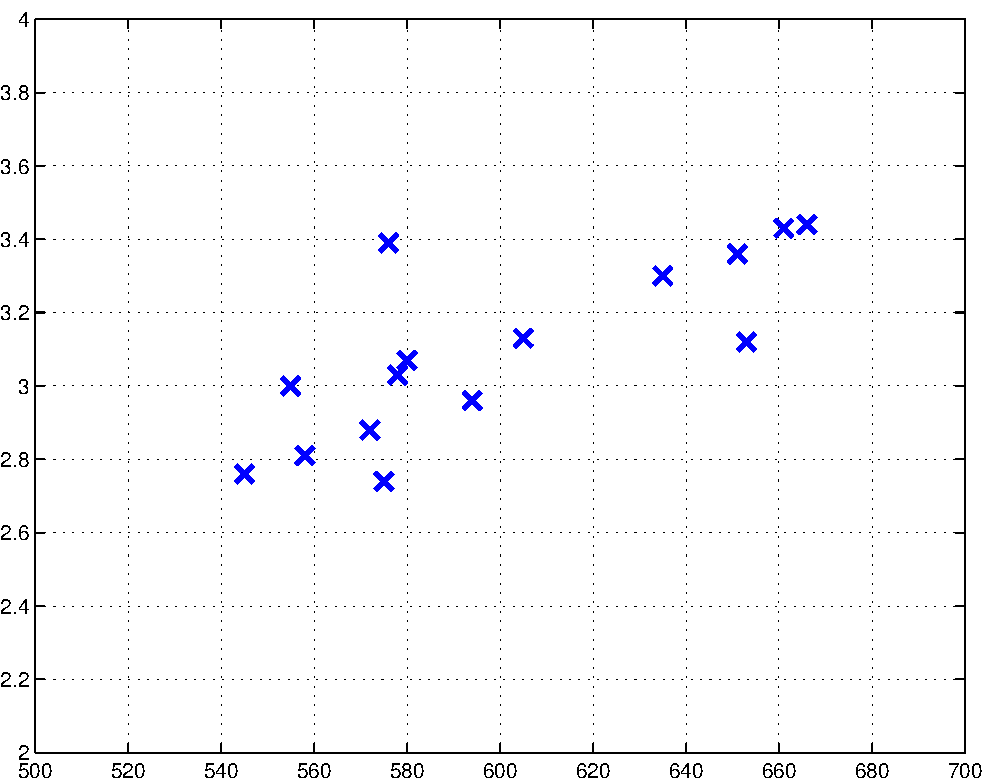
\includegraphics[width=.9\linewidth]{schoollsatgpa}
\end{figure}
\end{columns}

}
